IEEE $802.11$ networks use a shared and limited medium to establish communication among nodes. Carrier Sense Multiple Access with Collision Avoidance (CSMA/CA) is the protocol in charge of coordinating access to the wireless medium in order to avoid simultaneous transmissions by different nodes. If two or more nodes (or \emph{contenders} for the medium $N$) attempt transmission at the same time, a \emph{collision} accurs and the resulting transmission is disregarded by receivers.

Time in WLANs is slotted, that means that it is discrete and furthermore, it is divided in three slot types: \emph{empty}, \emph{successful} and \emph{collision}; accounting for no transmission, successful transmission or collision, respectively. 

Each contender attempting to transmit a packet chooses a uniformly random \emph{backoff} counter $bo_{r} \in [0,\ldots,CW_{min}-1]$, where $CW_{min}$ is referred to as the minimum \emph{contention window} with a typical value of $32$. Each passing empty slot decrements $bo_{r}$ by one; when the backoff counter reaches zero the contender will attempt transmission. The success of the transmission attempt is only confirmed by the reception of an \emph{acknowledgement} (\emph{ack}) from the receiver, otherwise a collision is assumed. If that were the case, each contender involved in the collision doubles its contention window $CW = 2^{m}CW_{min}, m\in[0,\ldots,5]$ incrementing the \emph{backoff stage} ($m$) by one and choosing another uniformly random backoff counter, $bo_{r}$. If the transmission is successful, the sender resets its contention window to the minimum value ($CW=CW_{min}$) and chooses another~$bo_{r}$.

Carrier Sense Multiple Access with Enhanced Collision Avoidance (CSMA/ECA) achieves less collisions and outperforms CSMA/CA in most typical scenarios~\cite{CSMA_ECA}. The only difference with CSMA/CA is that a deterministic backoff~$bo_{d} = C$ is chosen after each successful transmission. $C$ is defined in Eq.~\ref{eq:capacity} as the \emph{system capacity} and represents the maximum number of host ($N$) participating in the contend for transmission able to achieve a collision-free state. In Eq.~\ref{eq:capacity},~$\lceil{\cdotp}\rceil$ is the ceiling operator, $E[\cdotp]$ is the expectation operator, $\mathcal{U}$ is the uniform distribution and $CW$ is the contention window.

%Its evolution, CSMA/E2CA introduces stickiness in the process in order to shorten the convergence time towards a collision-free state by setting a number of occasions a deterministic backoff is used after each successful transmission~\cite{CSMA_ECA} .

%Stickiness can reduce the convergence time by orders of magnitude when the number of contenders $N$ is less or equal than the system capacity $C$ as defined in Eq.~\ref{eq:capacity}, where $\lceil{\cdotp}\rceil$ is the ceiling operator, $E[\cdotp]$ is the expectation operator, $\mathcal{U}$ is the uniform distribution and $CW_{min}$ is the minimum contention window of the system (usually $CW_{min}=32$ for 802.11 networks). 

\begin{equation} \label{eq:capacity}	
	C = \lceil{E[\mathcal{U}[0, CW - 1]]}\rceil
\end{equation}

In a scenario where $N \leq C$, eventually all contenders will be able to pick different transmission slots, therefore achieving a collision-free state.

When the system is overcrowded, $N>C$, CSMA/ECA suffers a decrease in throughput as appreciated in Figure~\ref{fig:throughput}. This effect is caused by collisions originated by $N-C$ contenders forced to generate a random backoff counter and attempting transmission on slots previously picked by $C$ nodes using a deterministic backoff.


\begin{figure}[htbp]
  \centering
  \includegraphics[width=0.7\linewidth, angle = -90]{figures/throughput/throughput.eps}
  \caption{Throughput and how it is affected when $N>C$
  \label{fig:throughput}}
\end{figure}

As $N-C$ nodes are unable to successfully transmit, collisions in turn force the $C$ nodes that chose a deterministic backoff, to switch to a random one. The resulting effect is a system where all nodes choose a random backoff (CSMA/CA), which do not take advantage of the higher throughput CSMA/ECA offers.

%The collision-free state is compromised when $N>C$. As more contenders are introduced, the system behavior tends to be more like CSMA/CA: nodes are forced to choose a random backoff thus degrading the performance.

In this work, a fully-distributed version of CSMA/ECA is presented and the throughput issue when $N>C$ is assessed.